\chapter{Thực hiện Dự án}
\label{chap:project_execution}

\section{Thu thập Dữ liệu}
\label{sec:data_acquisition}

\subsection{Nguồn Dữ liệu}
\label{sec:data_sources}

Dự án dùng một benchmark công khai, \textbf{UA-DETRAC} \cite{wen2020uadetrac}: $100$ video giao thông thật quay ở $25$~fps, độ phân giải $960 \times 540$ bởi các camera cố định đặt trên cao tại đường phố và nút giao, có chú thích box và danh tính cho mọi phương tiện. Đây là benchmark chuẩn cho bài toán theo dõi nhiều phương tiện từ góc nhìn giám sát, đúng bối cảnh của đồ án. Cách chia chính thức ($60$ chuỗi huấn luyện và $40$ chuỗi test) được giữ nguyên: $40$ chuỗi test chỉ dùng cho các lần chạy test đã khóa.

Hai sản phẩm dữ liệu khác được sinh từ cùng các video: (i) \emph{sự kiện che khuất} lấy mẫu từ quỹ đạo ground-truth (Giai đoạn~1, Mục~\ref{sec:data_augmentation}), và (ii) \emph{sự kiện detector} tạo ra bằng cách chạy YOLOv8n \cite{jocher2023yolov8} và tracker trực tuyến trên các video \emph{huấn luyện} (fine-tune Giai đoạn~2, Mục~\ref{sec:training_process}).

\subsection{Thu thập Dữ liệu}
\label{sec:data_collection}

Chú thích gốc được chuyển sang định dạng văn bản MOT bằng \texttt{scripts/convert\_detrac.py}. Bản mirror nguồn lưu các \emph{vùng bỏ qua} tĩnh (vùng người chú thích không gán nhãn, như bãi đỗ xe ở xa) dưới dạng các dòng của một track giả ($528\,798$ dòng có \texttt{target\_id}$=-1$). Chúng được tách thành $407$ đa giác bỏ qua, và $72\,714$ box phương tiện ($5.7\%$) có tâm nằm trong các vùng này bị loại, để mô hình không bao giờ phải tái liên kết một xe mà người chú thích đã bỏ qua.

\subsection{Gán nhãn Dữ liệu}
\label{sec:data_annotation}

Không cần gán nhãn thủ công: mọi box phương tiện trong UA-DETRAC đều mang danh tính quỹ đạo. Các danh tính này cung cấp nhãn huấn luyện cho mọi sự kiện che khuất (ứng viên nào, nếu có, là cùng xe với mỗi track bị mất) và ground truth cho mọi phép đánh giá. Với sự kiện detector (Giai đoạn~2) và các clip trình diễn, mỗi box YOLOv8n được ghép \emph{hậu kiểm} với một box ground-truth bằng thuật toán Hungarian với IoU $\ge 0.45$; nhãn hậu kiểm này chỉ dùng để chấm điểm và fine-tune, không bao giờ đi vào tracker.

\subsection{Thống kê Bộ dữ liệu}
\label{sec:dataset_stats}

Bảng~\ref{tab:dataset_stats} tóm tắt bộ dữ liệu sau làm sạch; các giá trị được tính lại từ các file đã chuyển đổi cho báo cáo này.

\begin{table}[htbp]
    \centering
    \caption{Thống kê UA-DETRAC sau làm sạch (\texttt{data/mot}, \texttt{data/stats.json})}
    \label{tab:dataset_stats}
    \begin{tabularx}{\textwidth}{l r X}
        \toprule
        \textbf{Thuộc tính} & \textbf{Giá trị} & \textbf{Ghi chú} \\
        \midrule
        Chuỗi video & $100$ & $60$ huấn luyện chính thức + $40$ test chính thức \\
        Khung hình có chú thích & $138\,045$ & $45\,603$ khung hình có $\ge 10$ xe \\
        Quỹ đạo phương tiện & $8\,251$ & Độ dài trung vị $86$ khung hình; $P_{10}=31$, $P_{90}=245$ \\
        Box phương tiện & $1\,201\,341$ & Trung bình $8.7$ xe mỗi khung hình; $0$ box người đi bộ \\
        Vùng bỏ qua & $407$ đa giác & Loại $72\,714$ box nằm trong đó \\
        Sự kiện validation & $6\,000$ & $11\,389$ track bị mất, cố định và đã băm \\
        Sự kiện test & $12\,000$ & $27\,120$ track bị mất, cố định và đã băm \\
        Sự kiện huấn luyện & $120\,038$ & Lấy mẫu từ $47$ chuỗi huấn luyện \\
        \bottomrule
    \end{tabularx}
\end{table}

\subsection{Chia Dữ liệu}
\label{sec:data_splitting}

Các video từ cùng một camera trông gần như giống hệt nhau, nên chia ngẫu nhiên theo video sẽ làm rò rỉ khung cảnh sang tập validation. Vì vậy \texttt{scripts/group\_locations.py} tính nền trung vị $64 \times 36$ cho mỗi chuỗi và gom các chuỗi bằng phân cụm agglomerative ($1-r \le 0.65$) thành $25$ cụm camera, gần với $\sim\!24$ địa điểm vật lý của UA-DETRAC. $60$ chuỗi huấn luyện được chia \emph{theo cụm} thành $47$ chuỗi huấn luyện ($13$ cụm) và $13$ chuỗi validation ($4$ cụm). $40$ chuỗi test chính thức được giữ nguyên; chúng thuộc $15$ cụm, trong đó $7$ cụm cũng có trong huấn luyện hoặc validation và $8$ cụm chưa từng thấy. Hai tập con được báo cáo riêng (Mục~\ref{sec:data_preprocessing}). Không dùng lật ngang hay bản sao phản chiếu ở bất kỳ đâu, vì lật ảnh sẽ tạo ra hướng lưu thông không thể có.

\subsection{Đạo đức và Quyền riêng tư}
\label{sec:ethics}

UA-DETRAC là benchmark nghiên cứu công khai. Hệ thống chỉ xử lý box phương tiện và histogram màu thô: không đọc biển số, không phát hiện khuôn mặt hay nhận dạng người, và detector trực tiếp được giới hạn ở các lớp phương tiện. Bảng điều khiển chỉ nêu các sự kiện \emph{có thể} xảy ra (lộ trình cấm, mất mục tiêu) để người vận hành xem xét; nó không đưa ra quyết định xử phạt. Các clip trình diễn là đoạn trích ngắn từ video test và chỉ dùng cho buổi trình bày.

\subsection{Hạn chế của Dữ liệu}
\label{sec:data_limitations}

UA-DETRAC gồm ô tô con, xe van, xe buýt và các xe lớn khác quay tại các thành phố Trung Quốc; bộ dữ liệu không có lớp xe máy, nên mô hình được huấn luyện và đánh giá mà không có xe máy. Mọi camera đều cố định và đặt trên cao, tập validation chỉ gồm bốn địa điểm camera, và tập test chính thức có chung $7$ trong $15$ địa điểm với tập huấn luyện. Các giới hạn này xác định phạm vi của kết luận (Mục~\ref{sec:limitations}).

\section{Phương pháp Huấn luyện}
\label{sec:training_methodology}

\subsection{Tổng quan Thành phần Được và Không được Huấn luyện}
\label{sec:trained_components}

Chỉ mạng tái liên kết được huấn luyện (Bảng~\ref{tab:trained_components}); phát hiện, các tầng tracking và quy tắc giám sát là thuật toán cố định hoặc mô hình bên ngoài.

\begin{table}[htbp]
    \centering
    \caption{Các thành phần được và không được huấn luyện}
    \label{tab:trained_components}
    \begin{tabularx}{\textwidth}{l c X}
        \toprule
        \textbf{Thành phần} & \textbf{Huấn luyện?} & \textbf{Cách tiếp cận} \\
        \midrule
        Tái liên kết GapLink-Lite & Có & Mạng tự phát triển, khởi tạo ngẫu nhiên, $327\,979$ tham số \\
        Checkpoint thích ứng detector (v1.3) & Có & Fine-tune từ mô hình đã đóng băng trên sự kiện detector của video huấn luyện \\
        Hiệu chuẩn $\sigma$ & Khớp tham số & Hệ số phụ thuộc khoảng trống $(a,b,c)$ khớp trên nửa~A validation \\
        Detector phương tiện & Không & YOLOv8n \cite{jocher2023yolov8}, dùng nguyên trạng (chỉ Giai đoạn~2 và demo) \\
        Tracking tầng 1 & Không & IoU + ghép Hungarian \cite{kuhn1955hungarian} \\
        Baseline C-1 \dots C-4 & Không & IoU, vận tốc không đổi, Kalman \cite{kalman1960} + Mahalanobis \cite{mahalanobis1936}, + kích thước và màu \\
        Quy tắc giám sát & Không & Đa giác vùng, logic lộ trình và khóa mục tiêu, chấm theo GT \\
        \bottomrule
    \end{tabularx}
\end{table}

\subsection{Lựa chọn Mô hình}
\label{sec:model_selection}

Cho $N \le 6$ track bị mất và $M \le 10$ detection ứng viên tại khung xác nhận $t_{\text{conf}}$, GapLink-Lite xuất ra một phép gán ngẫu nhiên kép (doubly stochastic) trên ma trận mở rộng $(N+1)\times(M+1)$, trong đó hàng và cột thêm vào (các \emph{dustbin}) hấp thụ track và ứng viên không được ghép. Năm module của mô hình (Hình~\ref{fig:model_arch}) được chọn để giải quyết ba thách thức ở Mục~\ref{sec:bg_challenges}:
\begin{enumerate}
    \item \textbf{Bộ mã hóa chuyển động.} Mỗi bước lịch sử của track bị mất được mô tả bằng đặc trưng bất biến tỉ lệ, chuẩn hóa theo chiều cao box cuối $h_l$ (độ dịch chuyển, vận tốc, log tỉ lệ kích thước). GRU 2 lớp \cite{cho2014gru} ($d=128$) mã hóa lịch sử, và khoảng trống $g_i = t_{\text{conf}} - t_{\text{lost},i}$ được embedding riêng để mô hình có thể mở rộng độ bất định khi khoảng trống dài.
    \item \textbf{Bộ mã hóa ngữ cảnh.} Tối đa $8$ xe lân cận tại $t_{\text{lost}}$ và $t_{\text{conf}}$ được mã hóa bằng MLP dùng chung và pooling max cộng mean bất biến hoán vị (DeepSets \cite{zaheer2017deepsets}).
    \item \textbf{Bộ dự đoán Gaussian.} Điểm neo vận tốc không đổi cộng phần dư học được cho vị trí dự đoán và log-phương sai đường chéo:
    \begin{equation}
        \mu_i = \hat{\mu}^{\text{CV}}_i + f_{\mu}(h_i, c_i, g_i), \qquad \ln \sigma_i^2 = \operatorname{clamp}\big(f_{\sigma}(h_i, c_i, g_i), -6, 4\big).
    \end{equation}
    \item \textbf{Bộ chấm điểm theo cặp và dustbin.} Với mỗi cặp track--ứng viên, log-mật độ Gaussian của ứng viên theo $(\mu_i, \sigma_i)$ được kết hợp với độ chồng lấn box, tỉ lệ kích thước và độ tương đồng cosine của histogram HSV vùng nhìn thấy thành logit $S_{ij}$. Logit dustbin của track và ứng viên nhận thêm độ gần biên ảnh và thống kê cạnh tranh, để mô hình có thể nói ``track này đã rời đi'' hoặc ``ứng viên này là xe mới'' \cite{sarlin2020superglue}.
    \item \textbf{Sinkhorn miền log.} $T=20$ lần chuẩn hóa xen kẽ hàng/cột \cite{sinkhorn1967,cuturi2013sinkhorn} với biên $\mathbf{r}=[1,\dots,1,M]$ và $\mathbf{c}=[1,\dots,1,N]$ cho ra $\log P$.
\end{enumerate}
Không cần mô hình lớn hơn: kiểm tra overfit trên 64 sự kiện đạt $100\%$ Top-1, và mô hình đầy đủ huấn luyện mất khoảng $100$~s mỗi lần chạy, cho phép chạy năm seed và ba ablation trong lịch trình.

\subsection{Môi trường Huấn luyện}
\label{sec:training_env}

Mọi thí nghiệm chạy cục bộ trên laptop có GPU NVIDIA GeForce RTX~3050 Laptop (6~GB VRAM), trong môi trường ảo Python~3.12 với PyTorch 2.11.0 (CUDA 12.8). Bảng~\ref{tab:train_hparams} liệt kê cấu hình huấn luyện được lưu trong checkpoint.

\begin{table}[htbp]
    \centering
    \caption{Siêu tham số huấn luyện}
    \label{tab:train_hparams}
    \begin{tabularx}{\textwidth}{l l X}
        \toprule
        \textbf{Tham số} & \textbf{Mô hình Giai đoạn 1} & \textbf{Fine-tune thích ứng detector (v1.3)} \\
        \midrule
        Trọng số ban đầu & Ngẫu nhiên (seed 20260417--21) & Checkpoint Giai đoạn~1 đã đóng băng \\
        Bộ tối ưu & AdamW \cite{loshchilov2019adamw}, lịch cosine có khởi động & AdamW \\
        Số bước / batch & $2\,400$ / $64$ sự kiện & $3\,000$ (tốt nhất ở $1\,500$) / $64$ \\
        Cắt gradient & $1.0$ & $1.0$ \\
        Mất mát & $\mathcal{L}_{\text{assign}} + 0.5\,\mathcal{L}_{\text{NLL}}$ & như trên \\
        Dữ liệu huấn luyện & $120\,038$ sự kiện GT & Trộn $70/30$ giữa $7\,746$ sự kiện detector và sự kiện GT \\
        Số lần chạy & 5 seed mô hình đầy đủ + 3 ablation $\times$ 5 seed & 1 seed (20261121) \\
        \bottomrule
    \end{tabularx}
\end{table}

\subsection{Tăng cường Dữ liệu}
\label{sec:data_augmentation}

Sự kiện huấn luyện được tổng hợp trực tiếp từ quỹ đạo ground-truth bởi \texttt{src/events.py}, đóng vai trò pipeline tăng cường dữ liệu:
\begin{itemize}
    \item \textbf{Độ dài che khuất.} Khoảng trống được lấy từ ba nhóm $3$--$15$, $16$--$45$ và $46$--$90$ khung hình với xác suất $0.4/0.4/0.2$.
    \item \textbf{Loại sự kiện.} Một track bị mất hoặc bị che rồi xuất hiện lại, hoặc bị detector bỏ sót, hoặc vắng mặt tại $t_{\text{conf}}$ vì đã rời khung hình hay vẫn còn bị che ($0.4/0.4/0.1/0.1$), để các dustbin được huấn luyện.
    \item \textbf{Nhiễu box.} Nhiễu vị trí Gaussian $3\%$ (lịch sử) và $5\%$ (ứng viên) kích thước box cùng dao động kích thước $\pm10\%$ mô phỏng box của detector; $5\%$ ứng viên đúng bị loại bỏ.
    \item \textbf{Che khuất một phần.} Với xác suất $0.4$, histogram màu của ứng viên chỉ lấy từ box con nhìn thấy (một trong bốn góc nhìn một phần tính sẵn), nên điểm ảnh bị che không bao giờ rò rỉ.
    \item \textbf{Curriculum.} Tỉ lệ sự kiện khó (có xe gây nhiễu gần hơn ứng viên đúng) tăng từ $0.40$ lên $0.75$ trong quá trình huấn luyện.
\end{itemize}
Không dùng phản chiếu và các biến đổi hình học khác của khung cảnh (Mục~\ref{sec:data_splitting}).

\subsection{Hàm Mất mát và Độ đo}
\label{sec:loss_metrics}

Mất mát gán là negative log-probability của phép gán đúng theo $P$, gồm cả các ô dustbin; mất mát dự đoán là Gaussian negative log-likelihood của vị trí xuất hiện lại thật. Đánh giá dùng các độ đo:
\begin{itemize}
    \item \textbf{Top-1 cấp sự kiện}: tỉ lệ track bị mất được gán đúng ứng viên hoặc được gán đúng vào dustbin; \textbf{WLR} (tỉ lệ liên kết sai): tỉ lệ được liên kết với ứng viên sai.
    \item \textbf{Độ phủ 90\%} và NLL 2D của ellipse dự đoán (hiệu chuẩn).
    \item \textbf{IRR} (tỉ lệ khôi phục danh tính): tỉ lệ khoảng che khuất mà sau đó xe giữ được ID trong tracker trực tuyến; \textbf{WLR}, \textbf{IDF1}, \textbf{MOTA} và \textbf{IDSW} ở cấp tracker.
    \item \textbf{Nat-IRR / Nat-WLR}: các độ đo tương tự trên khoảng trống tự nhiên của detector dài $3$--$95$ khung hình ở Giai đoạn~2.
\end{itemize}
Khoảng tin cậy là bootstrap ghép cặp \cite{efron1994bootstrap} với đơn vị lấy mẫu lại là địa điểm camera ($15$ địa điểm test, $10\,000$ lần rút).

\subsection{Quá trình Huấn luyện và Chọn Mô hình}
\label{sec:training_process}

Top-1 trên validation được đánh giá mỗi $600$ bước (Hình~\ref{fig:training_curves}); mất mát gán đã làm mượt giảm đến bước $1\,800$ và Top-1 validation đạt $93.2\%$ ở lần đánh giá cuối (bước $2\,400$), không có dấu hiệu overfit trên các địa điểm validation. Seed~1 được đóng băng thành \texttt{release/final.pt} (SHA-256 \texttt{844fc391\ldots}); bốn seed còn lại dùng cho trung bình $\pm$ độ lệch chuẩn và ablation.

\begin{figure}[htbp]
    \centering
    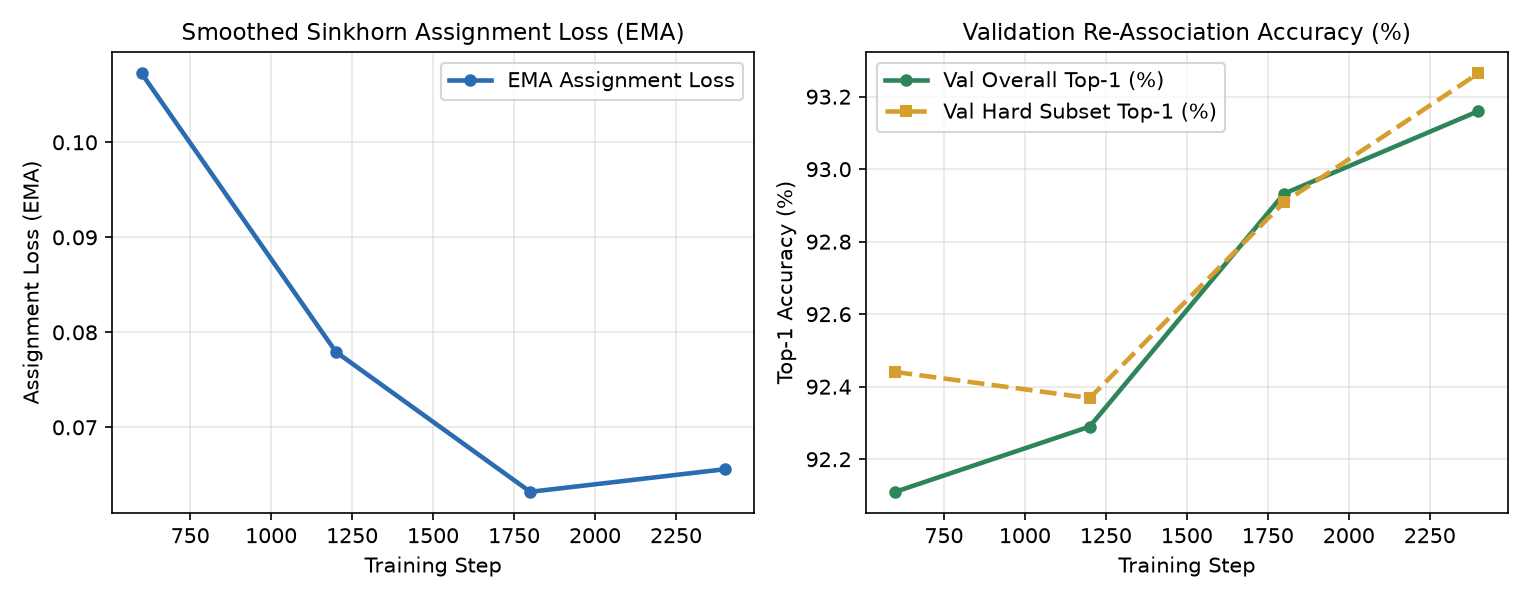
\includegraphics[width=0.95\textwidth]{figures/fig_training_curves.png}
    \caption{Huấn luyện mô hình đã đóng băng: mất mát gán đã làm mượt (trái) và độ chính xác Top-1 trên validation (phải), đánh giá mỗi 600 bước}
    \label{fig:training_curves}
\end{figure}

\textbf{Fine-tune theo detector.} Mô hình huấn luyện trên box ground-truth không bao giờ thấy độ rung của detector, hiện tượng chập chờn 2--5 khung hình hay ứng viên dương tính giả. Cho Giai đoạn~2, các sự kiện do tracker trực tuyến sinh ra trên detection YOLOv8n của các video \emph{huấn luyện} ($7\,746$ sự kiện) được gán nhãn hậu kiểm và dùng để fine-tune mô hình đã đóng băng. Checkpoint (\texttt{release/live\_v1.3.pt}, cùng kiến trúc) được chọn trên sự kiện detector của các video validation; video test không được dùng.

\subsection{Tinh chỉnh các Module Dựa trên Quy tắc}
\label{sec:rule_tuning}

Mọi ngưỡng đều được chọn trên dữ liệu validation và đóng băng trong \texttt{release/tracker.yaml} và \texttt{release/live\_v1.3.yaml}:
\begin{itemize}
    \item \textbf{Ngưỡng chấp nhận.} Liên kết $(i,j)$ của GapLink-Lite được chấp nhận khi và chỉ khi $P_{ij} \ge \tau$ và $P_{ij} > P_{i,\text{dustbin}}$. Giai đoạn~1: $\tau = 0.25$; Giai đoạn~2: $\tau = 0.65$ (Nat-IRR validation cao nhất với điều kiện Nat-WLR $\le 5\%$). Ngưỡng gating của baseline được chọn theo cùng quy tắc (trực tiếp: C-2 $\theta=1.2$, C-3 $\theta=1.0$, C-4 $\theta=1.2$).
    \item \textbf{Tracker.} Ngưỡng IoU tầng 1 là $0.30$; một track được xác nhận sau $3$ lần khớp; track bị mất được giữ $a_{\max} = 95$ khung hình, dài hơn khoảng trống dài nhất được chèn.
    \item \textbf{Hiệu chuẩn.} $\sigma' = \sigma \exp(a + b\ln(1+g) + c\ln^2(1+g))$ với $(a,b,c) = (0.413, -0.341, 0.074)$, khớp trên nửa~A của validation.
    \item \textbf{Chấm điểm demo.} Tái liên kết chỉ được chấm sau khoảng trống $\ge 3$ khung hình (cận dưới của các nhóm khoảng trống); box detector được ghép với ground truth ở IoU $\ge 0.45$.
\end{itemize}

\textbf{Tối ưu sau huấn luyện.} Bảng điều khiển được profile theo từng công đoạn trên ba clip với detection đã cache (script \texttt{bench\_vms\_fps.py}). Vì mô hình rất nhỏ, chạy trên GPU bị chi phối bởi overhead khởi chạy kernel: GapLink-Lite mất $17$--$23$~ms mỗi khung hình trên CUDA nhưng chỉ $8$--$9.5$~ms trên CPU với một luồng. Cùng với phép zoom rẻ hơn (cắt + resize tuyến tính thay cho affine warp bicubic) và chất lượng JPEG $80$, chi phí mỗi khung hình của bảng điều khiển giảm từ $69$--$83$~ms ($12$--$14.5$~FPS) xuống $22$--$28$~ms ($36$--$46$~FPS), cao hơn $25$~fps của video.

\section{Quy trình Hoạt động}
\label{sec:workflow}

\subsection{Tổng quan Hệ thống}
\label{sec:system_overview}

Hệ thống xử lý luồng video theo từng khung hình và giữ trạng thái giữa các khung (track đang hoạt động và bị mất, lịch sử vùng, mục tiêu đang khóa). Hình~\ref{fig:pipeline} thể hiện pipeline xử lý. Hai tracker chạy trên cùng detection, một với baseline và một với GapLink-Lite, nên mọi khác biệt trên màn hình chỉ đến từ module tái liên kết.

\begin{figure}[htbp]
    \centering
    \begin{tikzpicture}[
        node distance=0.42cm,
        st/.style={draw=SamsungBlue!80!black, rounded corners=3pt, fill=SamsungLightBlue!35, text width=8.6cm, align=center, minimum height=0.8cm, font=\small},
        dec/.style={draw=purple!60!black, diamond, aspect=2.6, fill=purple!6, text width=3.2cm, align=center, font=\small, inner sep=1pt},
        side/.style={draw=gray!60!black, rounded corners=3pt, fill=gray!8, text width=3.0cm, align=center, minimum height=0.8cm, font=\small},
        arr/.style={-{Stealth[length=2.2mm]}, thick}
    ]
        \node[st] (v) {Camera / file video (OpenCV)};
        \node[st, below=of v] (d) {Phát hiện phương tiện YOLOv8n + histogram HSV (cache sẵn cho clip demo)};
        \node[st, below=of d] (s1) {Tầng 1: ghép IoU + Hungarian cho các track đang hoạt động};
        \node[dec, below=of s1] (q) {Còn track bị mất và detection chưa ghép?};
        \node[st, below=0.5cm of q] (s2) {Tầng 2: tái liên kết --- GapLink-Lite (Sinkhorn + dustbin) hoặc baseline C-1\dots C-4};
        \node[st, below=of s2] (r) {Quy tắc giám sát: lộ trình cấm $Z_A\!\to\!Z_B$, khóa mục tiêu};
        \node[st, below=of r] (e) {Lớp phủ bảng điều khiển, bộ đếm, lịch sử sự cố (ảnh cắt trước/sau)};
        \node[side, right=0.9cm of q] (n) {Track mới / tiếp tục chờ};
        \node[side, right=0.9cm of e] (g) {Chấm hậu kiểm theo GT (chỉ để đánh giá)};
        \draw[arr] (v) -- (d); \draw[arr] (d) -- (s1); \draw[arr] (s1) -- (q);
        \draw[arr] (q) -- node[right, font=\small]{có} (s2); \draw[arr] (q) -- node[above, font=\small]{không} (n);
        \draw[arr] (s2) -- (r); \draw[arr] (r) -- (e); \draw[arr, dashed] (g) -- (e);
    \end{tikzpicture}
    \caption{Pipeline xử lý của tracker trực tuyến và bảng điều khiển GapLink-VMS}
    \label{fig:pipeline}
\end{figure}

\subsection{Tracking Trực tuyến Hai Tầng}
\label{sec:two_stage}

Tầng~1 ghép track đang hoạt động với detection có IoU $\ge 0.30$. Track không được ghép trở thành \emph{bị mất} và chờ tối đa $a_{\max} = 95$ khung hình. Tầng~2 chỉ chạy khi có track bị mất với tuổi $2$--$95$ khung hình và có detection chưa được ghép; nó tạo một sự kiện cho mỗi nhóm gồm tối đa $6$ track bị mất và $10$ ứng viên rồi gọi bộ ghép (associator) đã chọn. Detection chưa ghép khởi tạo track mới. Huấn luyện và tracking tạo sự kiện bằng cùng một hàm (\texttt{assemble\_event}, được kiểm tra bởi \texttt{tests/test\_parity.py}), nên không có sai lệch train--test trong định dạng sự kiện.

\subsection{Quyết định Tái liên kết}
\label{sec:reassoc_decision}

Với GapLink-Lite, phép ghép Hungarian trên $-P_{1:N,1:M}$ đề xuất các cặp, và một cặp chỉ được chấp nhận nếu
\begin{equation}
    P_{ij} \ge \tau \quad\text{và}\quad P_{ij} > P_{i,M+1},
\end{equation}
tức là khi liên kết có khả năng cao hơn ``chưa liên kết''. Ngược lại, track tiếp tục chờ (dustbin). Các baseline Kalman chấp nhận một cặp khi khoảng cách Mahalanobis $d^2_{ij} = \sum_{k\in\{x,y\}} (c_{jk} - \mu_{ik})^2 / \sigma_{ik}^2$ nhỏ hơn ngưỡng $\theta$ của chúng (cộng thêm thành phần kích thước và màu với C-4).

\subsection{Quy tắc Giám sát}
\label{sec:surveillance_rules}

\textbf{Lộ trình cấm.} Một track có vùng đầu tiên là $Z_A$ và sau đó đi vào $Z_B$ sẽ phát cảnh báo vi phạm. Với ground truth, mỗi vi phạm được chấm là \emph{đúng ID} (cùng một xe ở $Z_A$ và $Z_B$), \emph{sai ID} (xe ở $Z_B$ đúng là đến từ $Z_A$ nhưng ID của cảnh báo bắt đầu trên một xe khác) hoặc \emph{giả} (xe ở $Z_B$ chưa từng ở $Z_A$).

\textbf{Khóa mục tiêu.} Người vận hành click vào một xe; bảng điều khiển bám theo ID của xe đó. Khi mục tiêu bị che, vị trí dự đoán ($\mu$ của GapLink-Lite hoặc dự đoán Kalman) được vẽ thành đường nét đứt; khi một xe xuất hiện lại, mục tiêu được \emph{bắt lại} nếu là cùng xe và \emph{sai xe} nếu ngược lại.

\subsection{Lịch sử Sự cố}
\label{sec:incident_history}

Chỉ những sự kiện người vận hành cần kiểm tra mới được ghi: liên kết sai, xe bị gán ID mới, vi phạm lộ trình và mục tiêu bị mất hoặc sai. Mỗi mục lưu ảnh cắt của xe trước và sau sự kiện, phương pháp, ID và thời điểm, để người xem có thể nhận ra ngay hai ảnh có cùng một xe hay không.

\subsection{Giao thức Đánh giá và Đóng băng Kết quả}
\label{sec:eval_protocol}

Giả thuyết và giao thức được đăng ký trong \texttt{docs/PREREG.md} trước mọi lần chạy test. Ngưỡng chỉ được chọn trên validation; sự kiện test và video test được đánh giá một lần từ các checkpoint có băm SHA-256; kết quả được sao chép vào \texttt{release/results\_v1.1} và \texttt{release/results\_v1.3} kèm manifest đóng băng được kiểm tra bởi \texttt{scripts/freeze\_results.py}. Mọi sai lệch so với kế hoạch (gồm một lần chạy lại test Giai đoạn~1 sau khi sửa lỗi chuyển đổi dữ liệu) được ghi trong \texttt{docs/DEVIATIONS.md}.

\subsection{Quy trình Người dùng}
\label{sec:user_workflow}

Người vận hành chọn một trong ba clip, phát hoặc chạy từng khung hình, và đọc hai khung song song. Với nhiệm vụ lộ trình, các vùng $Z_A$ và $Z_B$ có thể được vẽ lại trên khung hình và lưu cùng clip; với nhiệm vụ mục tiêu, người vận hành tạm dừng và click vào một xe. Bảng kết quả và lịch sử sự cố cập nhật trực tiếp.

\subsection{Chế độ Hoạt động}
\label{sec:operating_modes}

Bảng điều khiển (\texttt{demo/vms\_lite.py}) có ba chế độ: dashboard web tương tác; \texttt{--check}, chạy ba clip không có giao diện và ghi độ đo vào \texttt{runs/vms\_lite\_check/metrics.json}; và \texttt{--render}, ghi các file MP4 song song có quay chậm ở những thời điểm then chốt làm phương án dự phòng cho buổi trình bày.

\section{Thiết kế Hệ thống}
\label{sec:system_design}

Hình~\ref{fig:sys_arch} thể hiện kiến trúc tổng thể của bảng điều khiển và Hình~\ref{fig:model_arch} thể hiện cấu trúc bên trong của GapLink-Lite.

\begin{figure}[htbp]
    \centering
    \resizebox{\textwidth}{!}{%
    \begin{tikzpicture}[
        box/.style={draw=SamsungBlue!80!black, rounded corners=4pt, fill=SamsungLightBlue!35, text width=2.7cm, align=center, minimum height=1.2cm, font=\small},
        gl/.style={draw=green!50!black, rounded corners=4pt, fill=green!8, text width=2.7cm, align=center, minimum height=1.2cm, font=\small},
        ext/.style={draw=gray!60!black, rounded corners=4pt, fill=gray!8, text width=2.7cm, align=center, minimum height=1.2cm, font=\small},
        arr/.style={-{Stealth[length=2.3mm]}, thick}
    ]
        \node[ext] (vid) at (0,0) {Clip video\\ \scriptsize\texttt{demo/sample\_videos}};
        \node[ext] (det) at (3.4,0) {YOLOv8n boxes + HSV\\ \scriptsize cache \texttt{\_dets.npz}};
        \node[box] (t1) at (7.2,1.0) {Tracker A\\ \scriptsize Stage 1 + C-3 Kalman};
        \node[gl] (t2) at (7.2,-1.0) {Tracker B\\ \scriptsize Stage 1 + GapLink-Lite};
        \node[box] (j) at (11.0,0) {Bộ chấm\\ \scriptsize tái liên kết, lộ trình, khóa};
        \node[ext] (gt) at (11.0,-2.4) {Ground truth\\ \scriptsize \texttt{\_gt.npz} (chỉ để chấm)};
        \node[box] (srv) at (14.6,0) {FastAPI server\\ \scriptsize luồng SSE, thao tác};
        \node[ext] (ui) at (18.0,0) {Trình duyệt web\\ \scriptsize khung hình, bảng, lịch sử};
        \draw[arr] (vid) -- (det); \draw[arr] (det) -- (t1); \draw[arr] (det) -- (t2);
        \draw[arr] (t1) -- (j); \draw[arr] (t2) -- (j); \draw[arr, dashed] (gt) -- (j);
        \draw[arr] (j) -- (srv); \draw[arr] (srv) -- (ui);
        \draw[arr] (ui.south) to[bend left=25] node[below, font=\scriptsize]{vùng, click để khóa, tua} (srv.south);
    \end{tikzpicture}%
    }
    \caption{Kiến trúc tổng thể của bảng điều khiển trình diễn GapLink-VMS}
    \label{fig:sys_arch}
\end{figure}

\begin{figure}[htbp]
    \centering
    \resizebox{\textwidth}{!}{%
    \begin{tikzpicture}[
        node distance=0.9cm and 1.1cm,
        box/.style={draw=SamsungBlue!80!black, rounded corners=4pt, fill=SamsungLightBlue!35, text width=3.1cm, align=center, minimum height=1.35cm, font=\small},
        inp/.style={draw=gray!70!black, rounded corners=4pt, fill=gray!10, text width=2.9cm, align=center, minimum height=1.35cm, font=\small},
        outb/.style={draw=red!65!black, rounded corners=4pt, fill=red!6, text width=3.2cm, align=center, minimum height=2.2cm, font=\small},
        arr/.style={-{Stealth[length=2.5mm]}, thick, draw=black!75}
    ]
        \node[inp] (lost) {\textbf{Track bị mất ($1\dots N$)}\\ \scriptsize box ($K\le 20$), khoảng trống $g_i$,\\ HSV EMA, ngữ cảnh tại $t_{\text{lost}}$};
        \node[inp, below=1.1cm of lost] (cand) {\textbf{Ứng viên ($1\dots M$)}\\ \scriptsize detection chưa ghép,\\ HSV vùng nhìn thấy, ngữ cảnh tại $t_{\text{conf}}$};
        \node[box, right=1.0cm of lost] (mot) {\textbf{1. Mã hóa chuyển động}\\ \scriptsize GRU 2 lớp ($d=128$)\\ + embedding khoảng trống};
        \node[box, right=1.0cm of cand] (ctx) {\textbf{2. Mã hóa ngữ cảnh}\\ \scriptsize DeepSets,\\ pooling max + mean};
        \node[box, fill=green!8, draw=green!55!black, right=1.0cm of mot] (pred) {\textbf{3. Dự đoán Gaussian}\\ \scriptsize neo CV + phần dư\\ $\rightarrow (\mu_i, \ln\sigma_i^2)$};
        \node[box, fill=purple!8, draw=purple!60!black, right=1.0cm of ctx] (scor) {\textbf{4. Theo cặp \& dustbin}\\ \scriptsize logit $S_{ij}$, track $z^t_i$,\\ ứng viên $z^c_j$};
        \node[outb, right=1.0cm of $(pred.east)!0.5!(scor.east)$] (sink) {\textbf{5. Log-Sinkhorn ($T=20$)}\\ \scriptsize ma trận $(N+1)\times(M+1)$ $P$\\ Hungarian + ngưỡng $\tau$\\ $\rightarrow$ tái liên kết hoặc chờ};
        \draw[arr] (lost) -- (mot); \draw[arr] (cand) -- (ctx); \draw[arr] (lost.south east) -- (ctx.north west);
        \draw[arr] (mot) -- (pred); \draw[arr] (ctx) -- (scor); \draw[arr] (ctx.north east) -- (pred.south west);
        \draw[arr] (mot.south east) -- (scor.north west); \draw[arr] (pred) -- (scor);
        \draw[arr] (pred.east) -- (sink.west |- pred.east); \draw[arr] (scor.east) -- (sink.west |- scor.east);
    \end{tikzpicture}%
    }
    \caption{Kiến trúc GapLink-Lite ($327\,979$ tham số) dùng ở Tầng 2}
    \label{fig:model_arch}
\end{figure}
